\قسمت{بررسی تاثیر تعداد نواحی محیط در کیفیت و سرعت یادگیری عامل‌ها در روش پیشنهادی}
همانطور که در تعریف
\ref{experties_definition}
آورده شده است، بنا به معیار خبرگی معرفی شده در این پژوهش باید محیط به تعدادی ناحیه افزار شود و سپس میزان حضور عامل در هر ناحیه را سنجیده و خبرگی عامل معکوسی از میزان حضور عامل در این نواحی می‌باشد. لذا ضروری است که در این قسمت به بررسی تاثیر تعداد نواحی محیط در کیفیت و سرعت یادگیری عامل‌ها در روش پیشنهادی بپردازیم.

\زیرقسمت{محیط پلکان مارپیچ}
ما محیط پلکان مارپیچ را به ۶ ناحیه‌ی مختلف با اندازه‌های
1$\times$1, 2$\times$2, $\cdots$ 6$\times$6
(کل محیط) تقسیم‌بندی کرده‌ایم و همان‌طور که در شکل
\ref{fig:maze_refsize_effect}
آمده است اندازه‌ی این نواحی در کیفیت و سرعت یادگیری روش پیشنهادی تفاوتی ایجاد نمی‌کند و می‌توان برای کل محیط را یک ناحیه فرض کرد و میزان خبرگی کلی عامل برابر می‌شود با تعداد گام‌هایی که عامل برای رسیدن به هدف طی می‌کند.

\begin{figure}
\centering
\caption{تاثیر ناحیه‌بندی‌ مختلف بروی کیفیت و سرعت یادگیری در محیط پلکان مارپیچ}\label{fig:maze_refsize_effect}
\begin{tabular}{*2c}
\subf{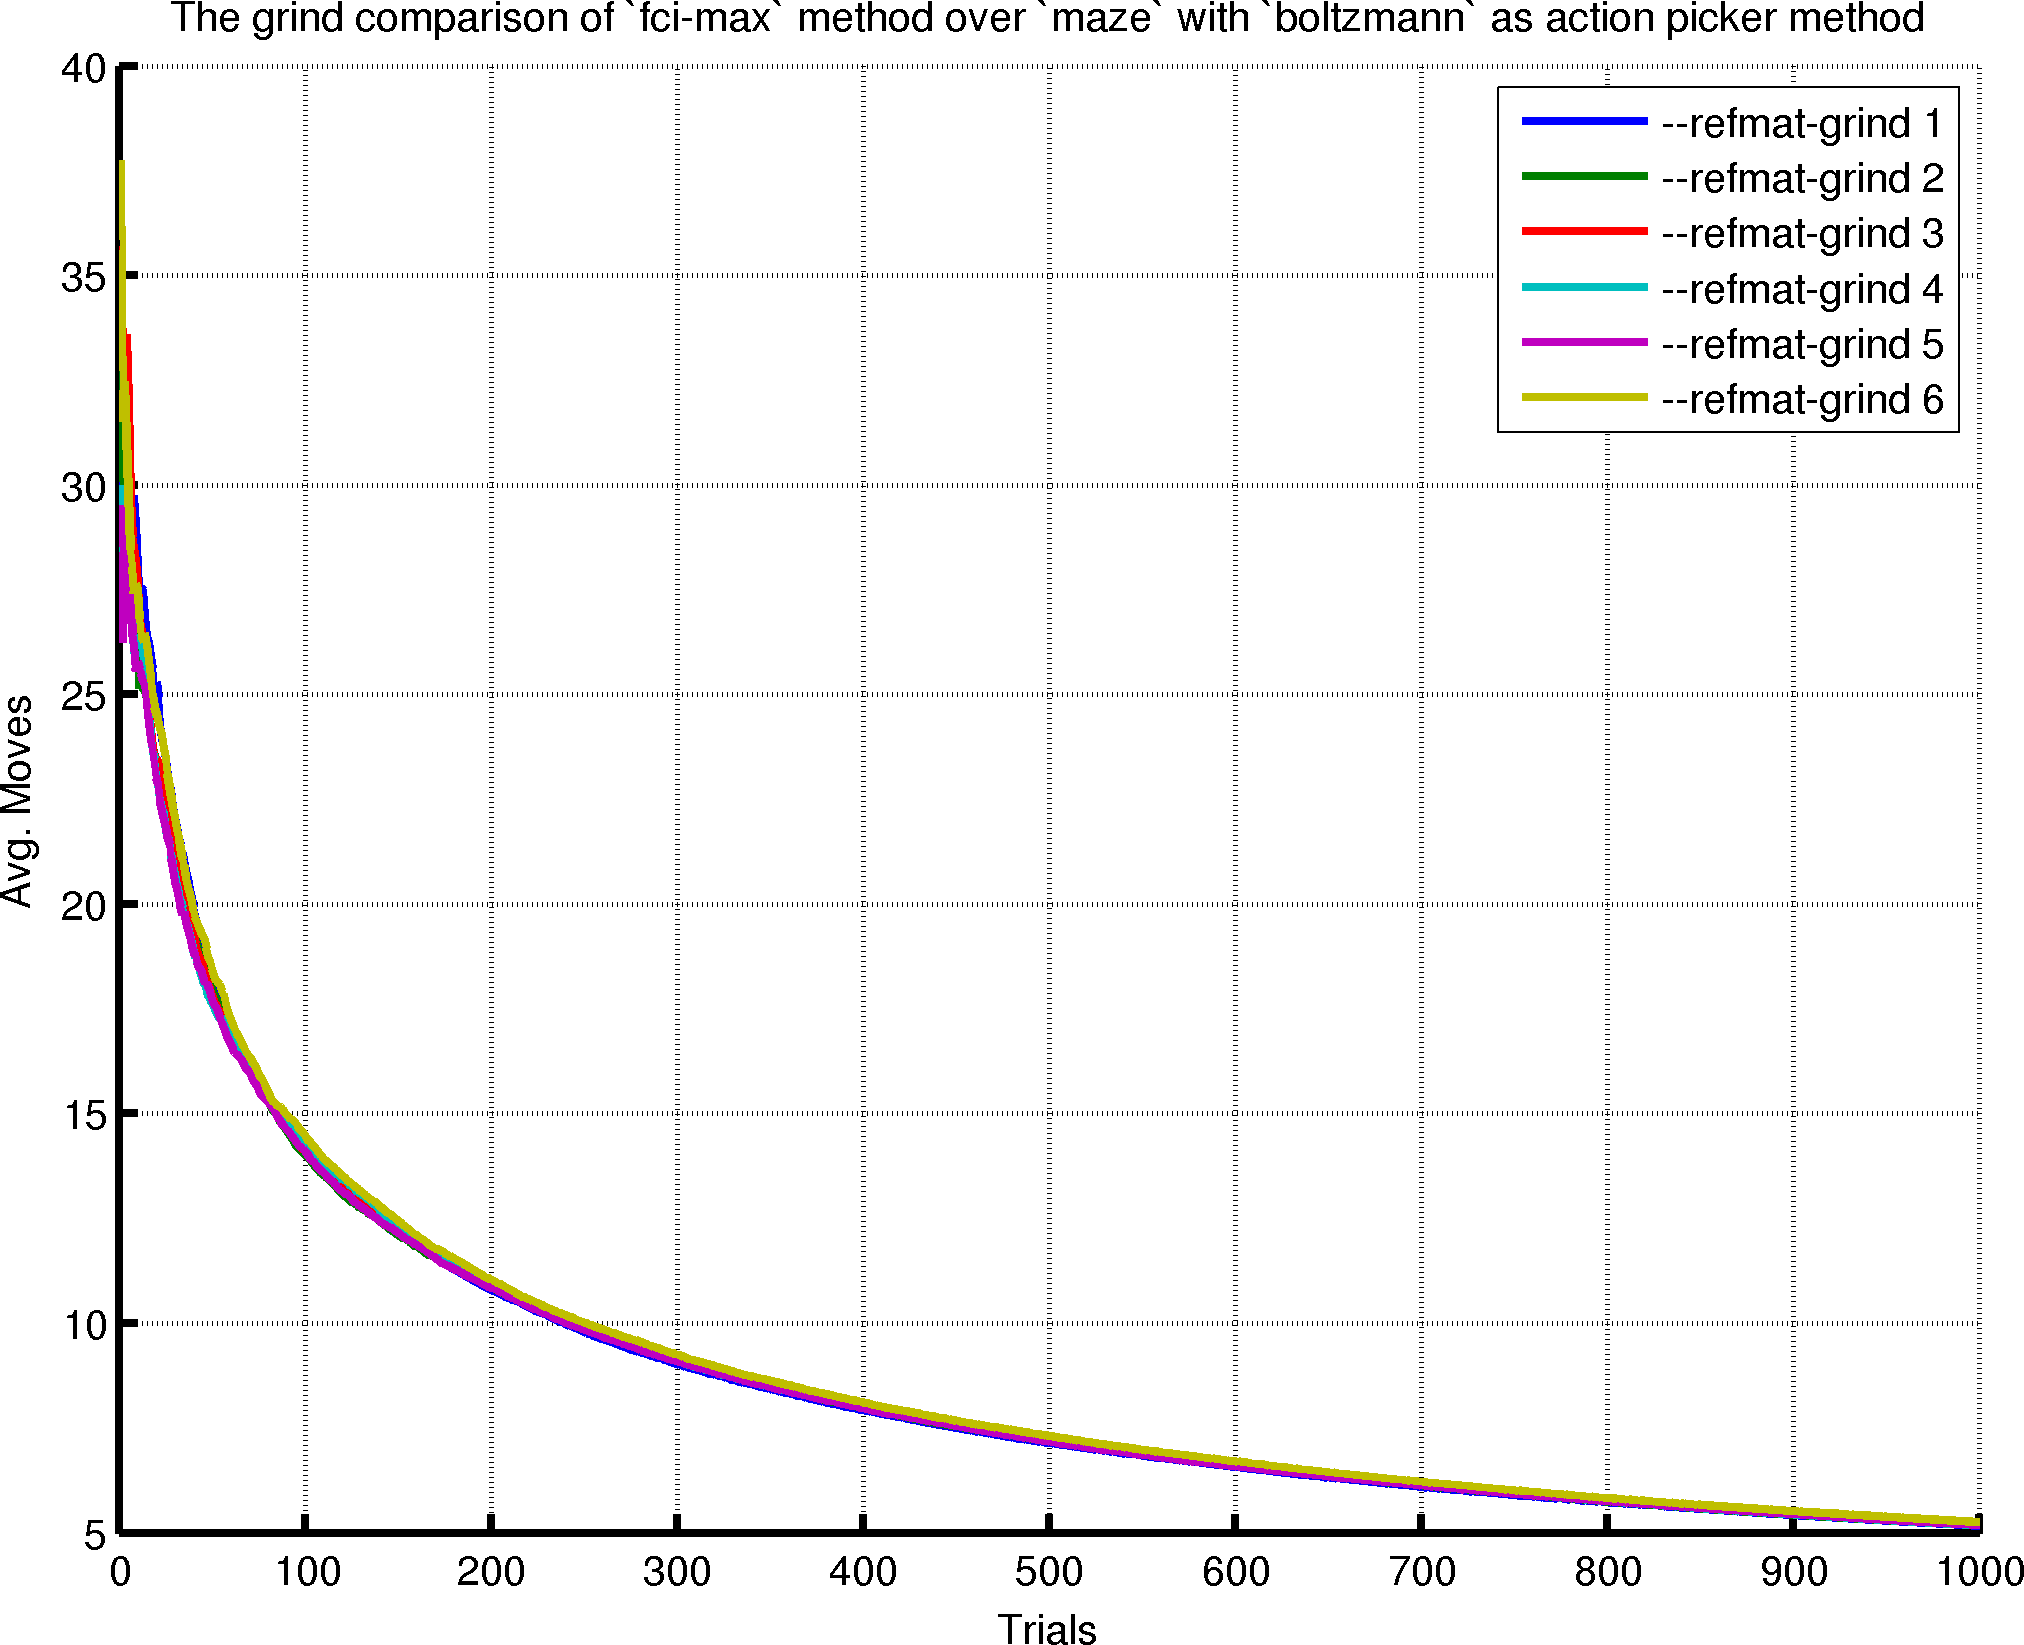
\includegraphics[width=.47\textwidth]{boltzmann/pref/refmat/env/maze/fci-max/maze-fci-max-grind-compare.png}}
     {\lr{Max($\cdot$)}}
&
\subf{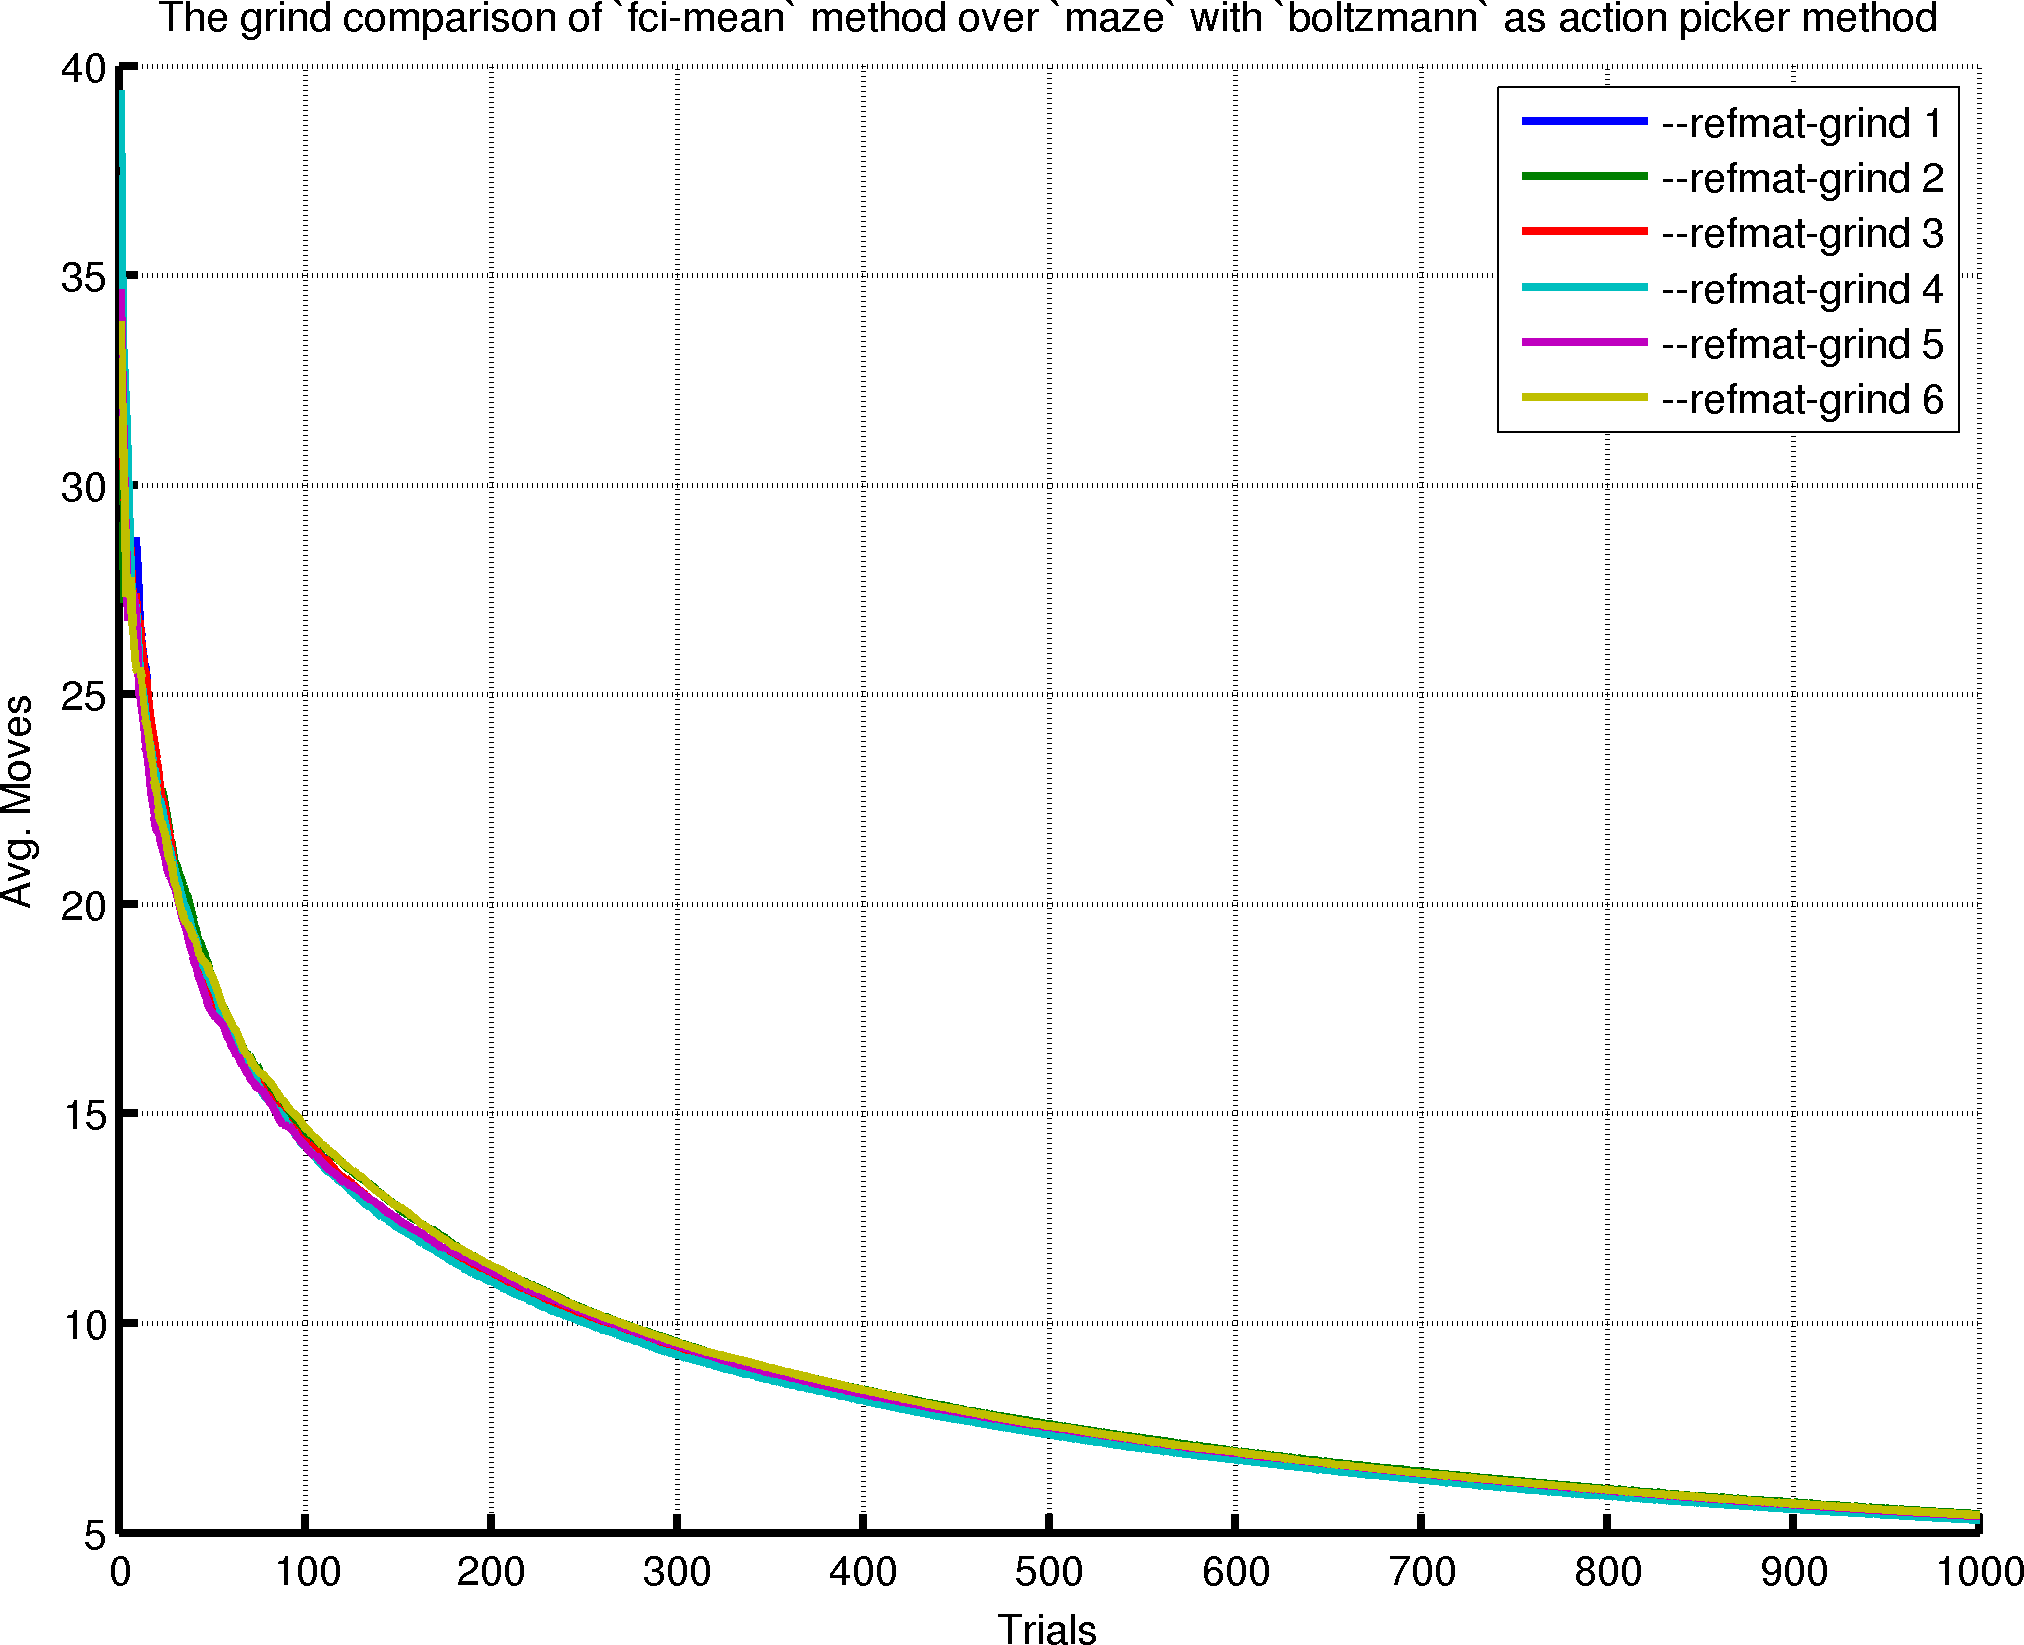
\includegraphics[width=.47\textwidth]{boltzmann/pref/refmat/env/maze/fci-mean/maze-fci-mean-grind-compare.png}}
     {\lr{Mean($\cdot$)}}
\\
\subf{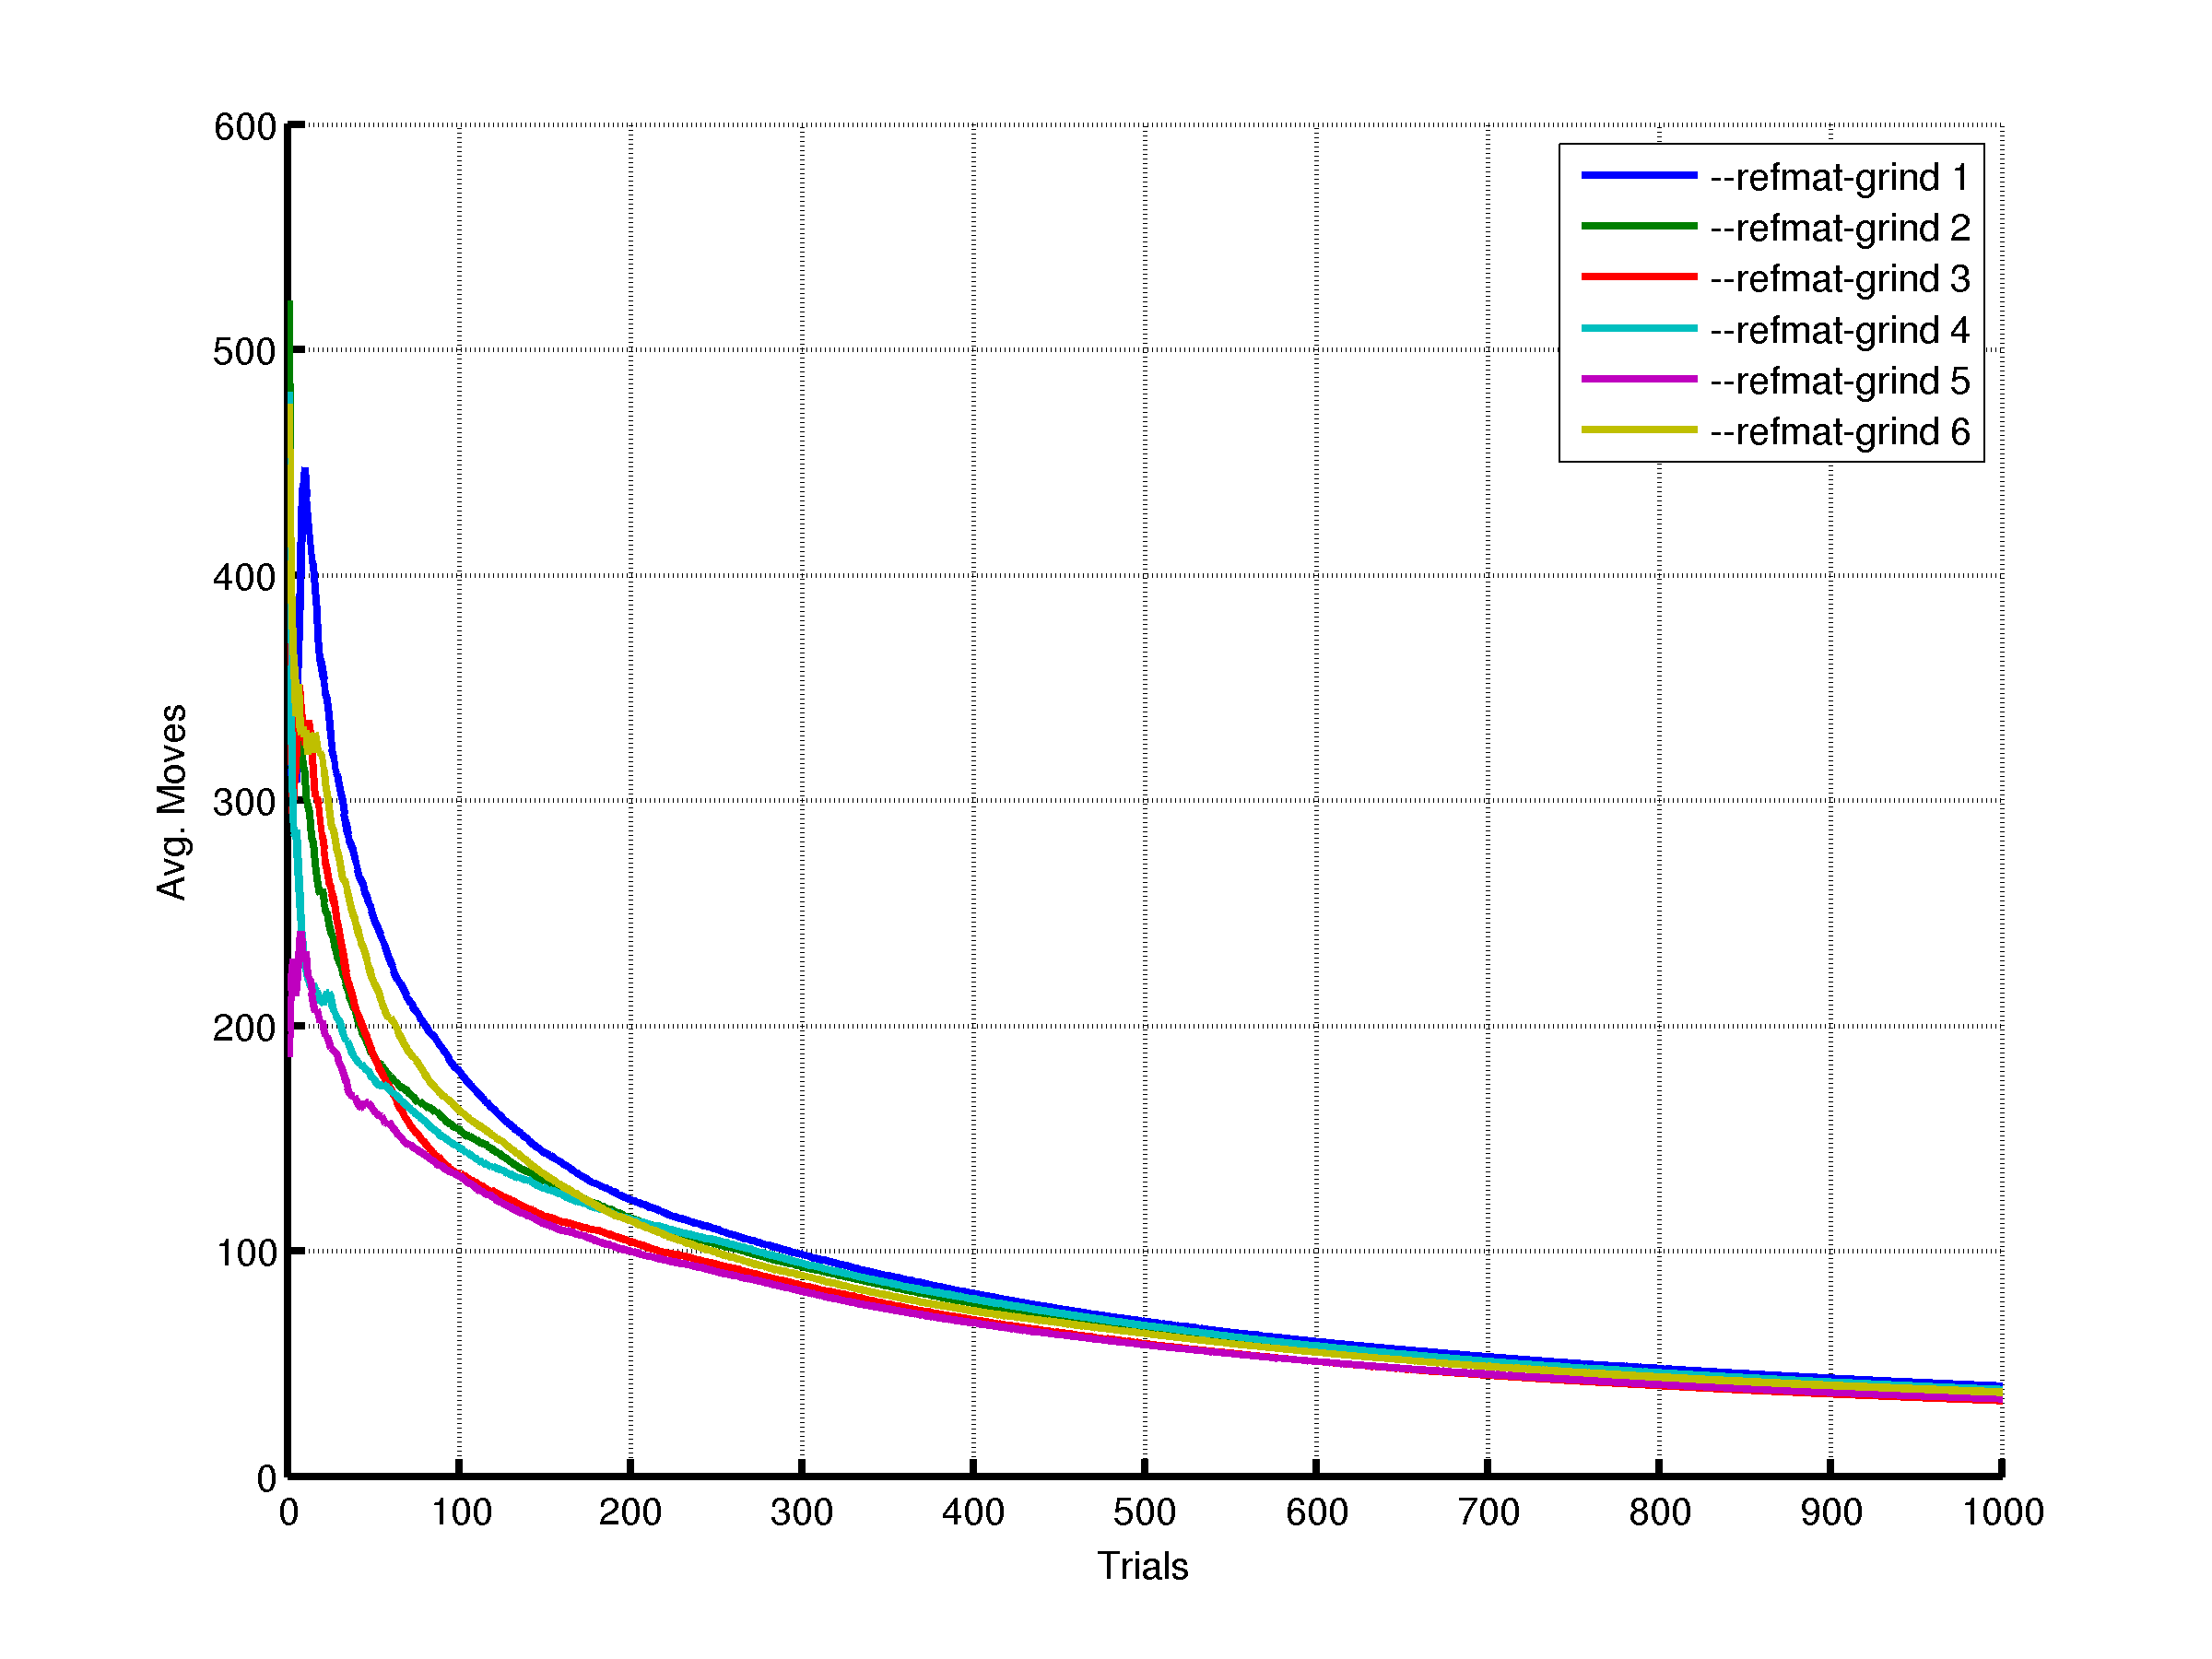
\includegraphics[width=.47\textwidth]{boltzmann/pref/refmat/env/maze/fci-k-mean/maze-fci-k-mean-grind-compare.png}}
     {\lr{K-Mean($\cdot$)}}
&
\subf{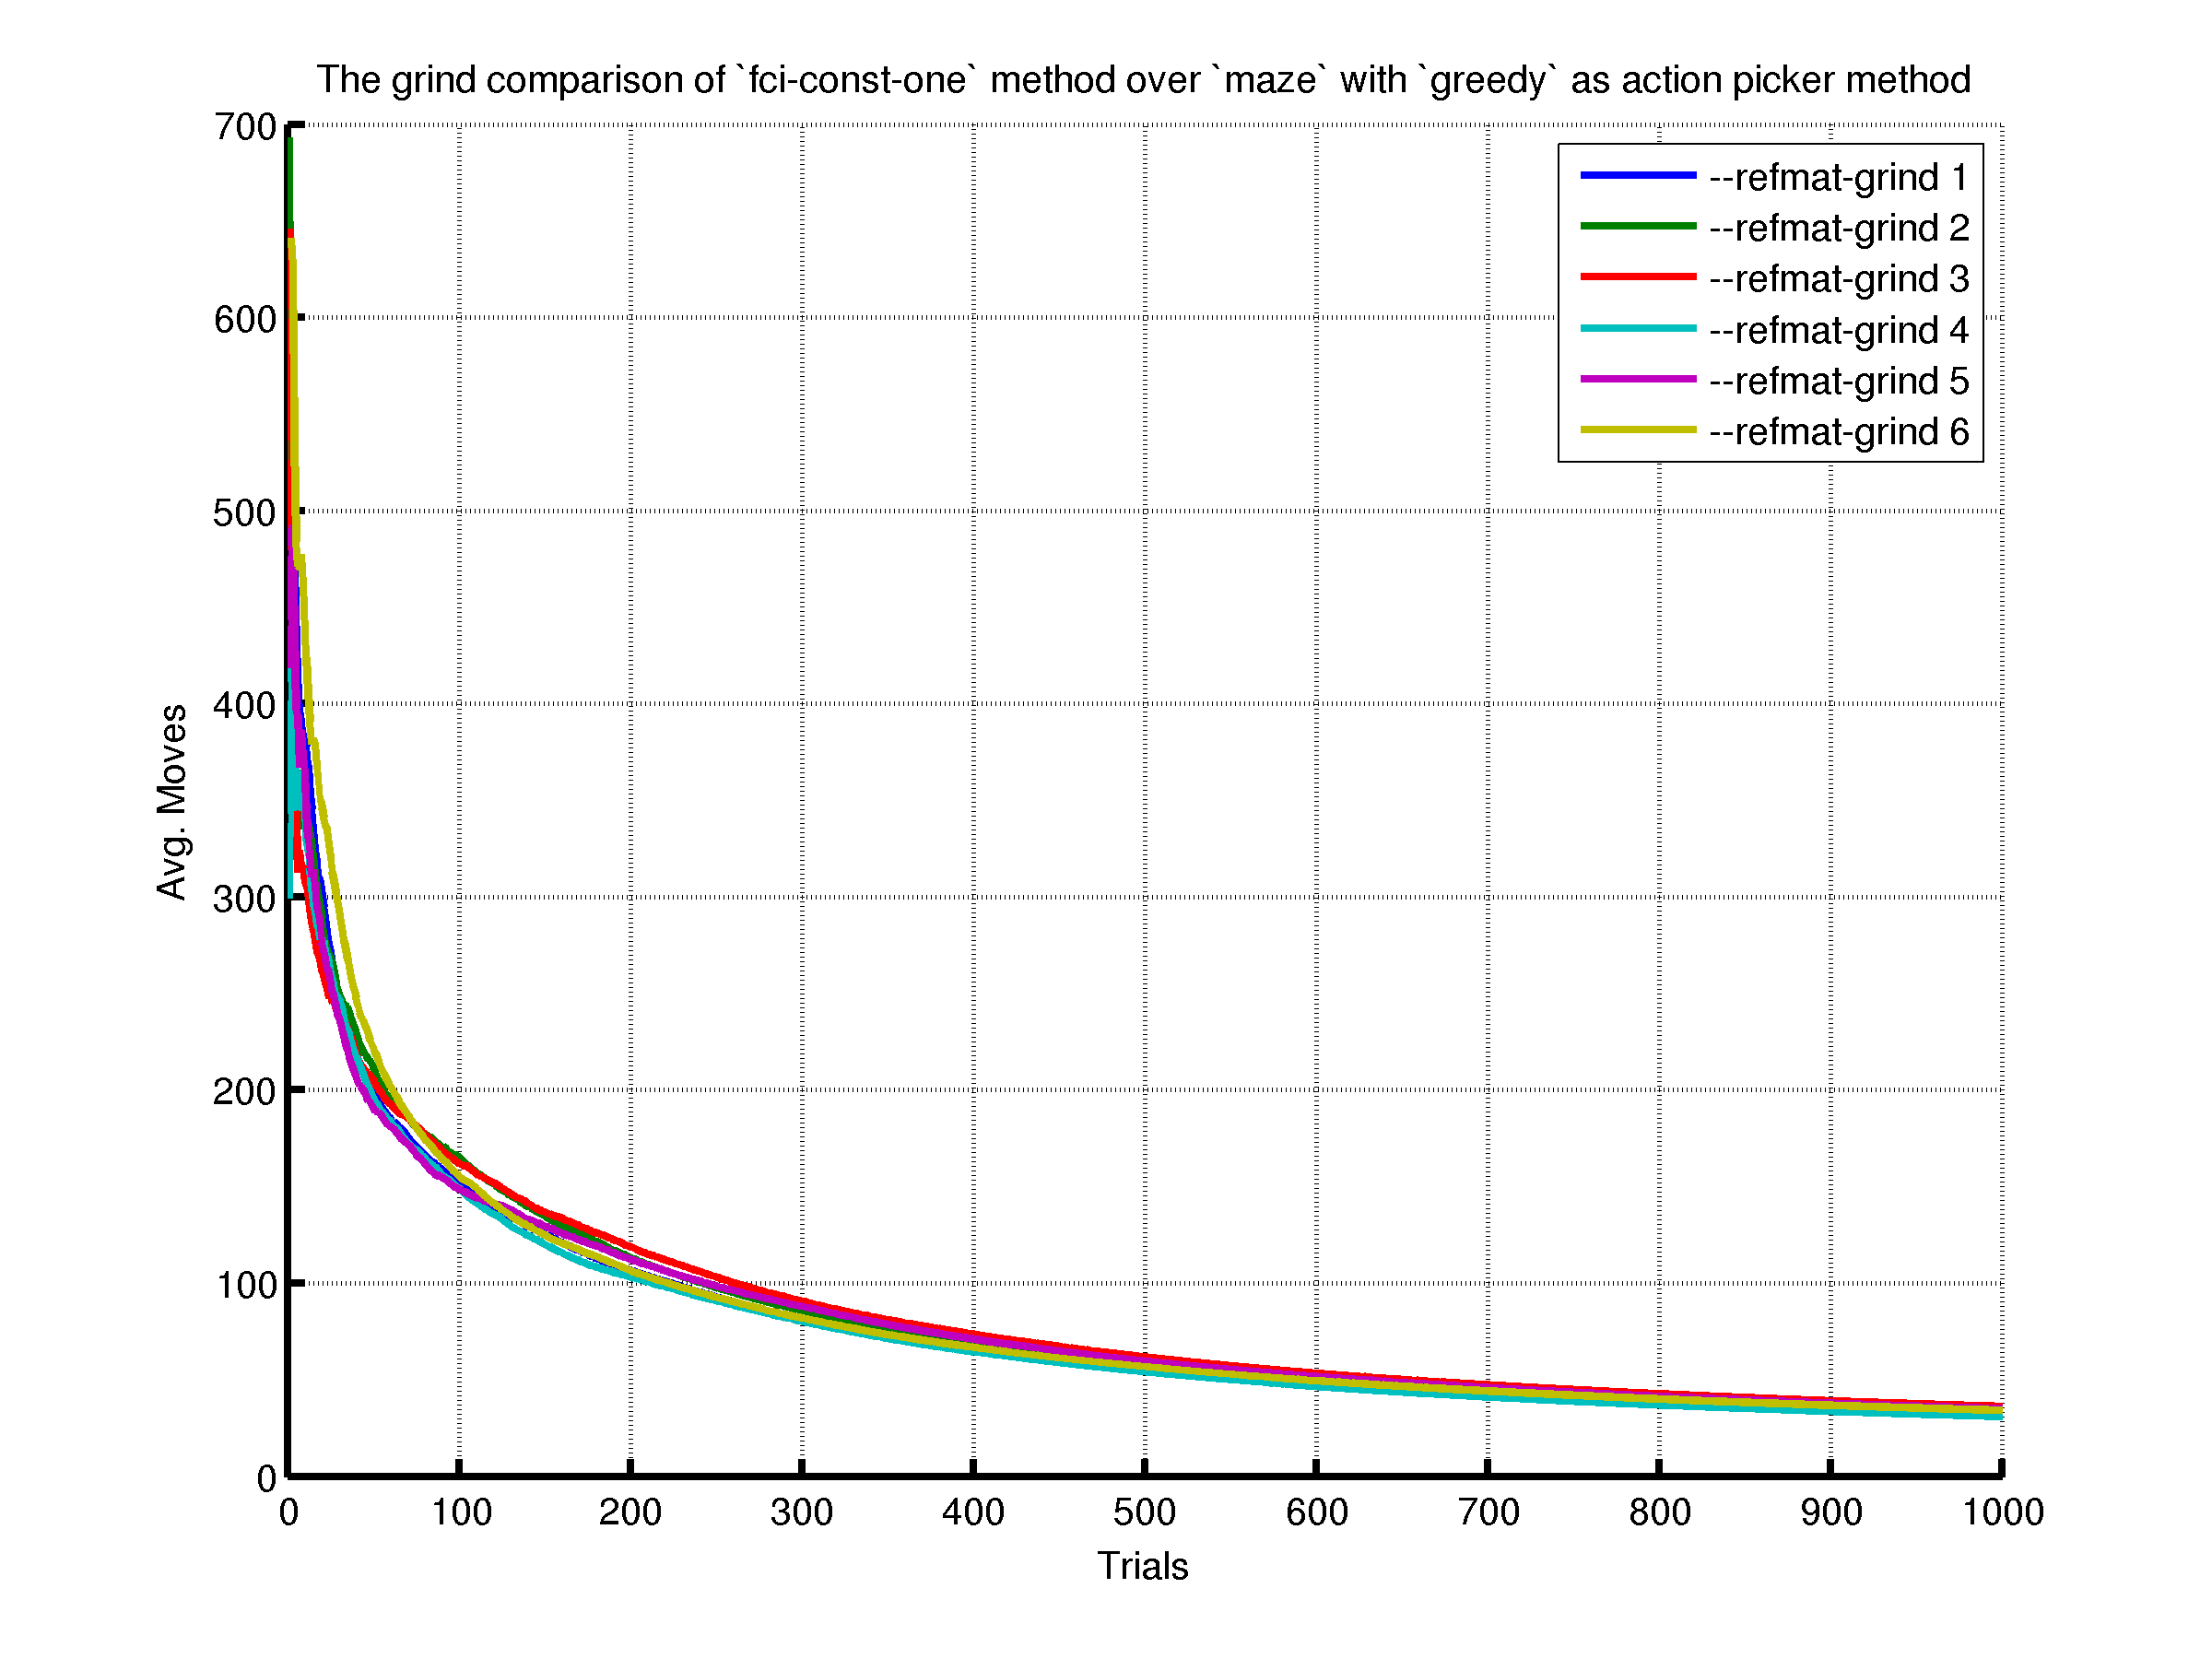
\includegraphics[width=.47\textwidth]{boltzmann/pref/refmat/env/maze/fci-const-one/maze-fci-const-one-grind-compare.png}}
     {\lr{Const-One($\cdot$)}}
\\
\end{tabular}
\end{figure}

\زیرقسمت{محیط پلکان صید و صیاد}
همانند محیط پلکان مارپیچ را به چند ناحیه‌ی مختلف با اندازه‌های
1$\times$1 $\cdots$ 17$\times$17
(کل محیط) تقسیم‌بندی کرده‌ایم و همان‌طور که در شکل
\ref{fig:prey_refsize_effect}
آمده است همچون محیط پلکان مارپیچ اندازه‌ی این نواحی در کیفیت و سرعت یادگیری روش پیشنهادی تفاوتی ایجاد نمی‌کند.

\begin{figure}
\centering
\caption{تاثیر ناحیه‌بندی‌ مختلف بروی کیفیت و سرعت یادگیری در محیط صید و صیاد}\label{fig:prey_refsize_effect}
\begin{tabular}{*2c}
\subf{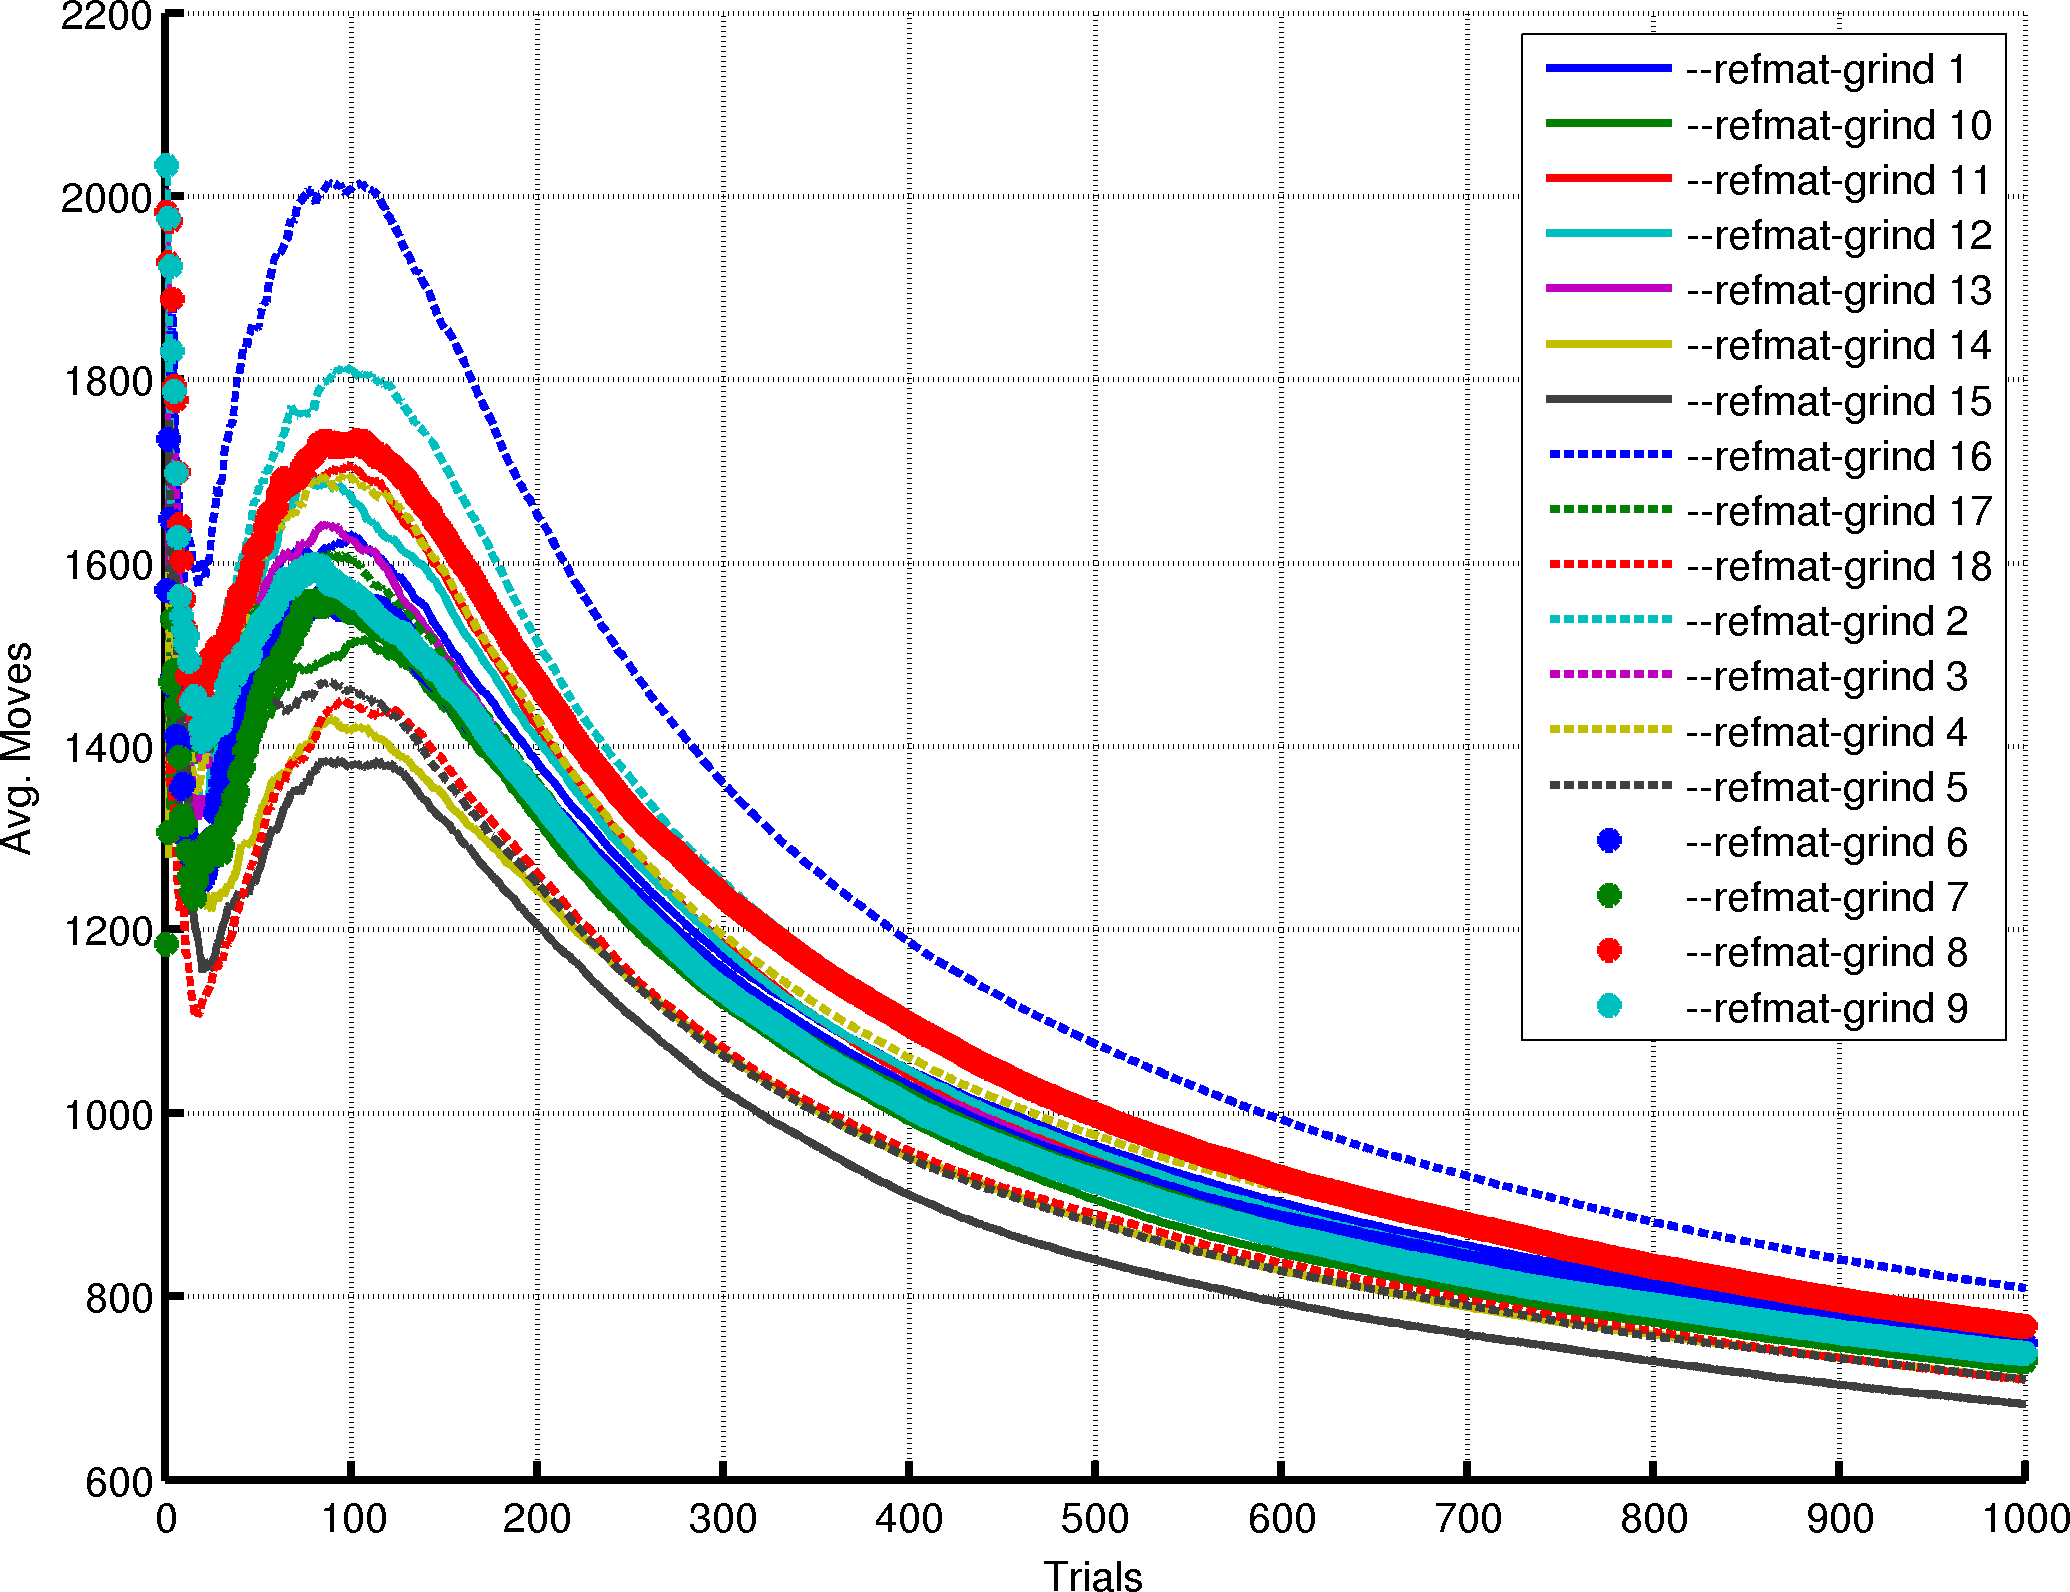
\includegraphics[width=.47\textwidth]{boltzmann/pref/refmat/env/prey/fci-max/prey-fci-max-grind-compare.png}}
     {\lr{Max($\cdot$)}}
&
\subf{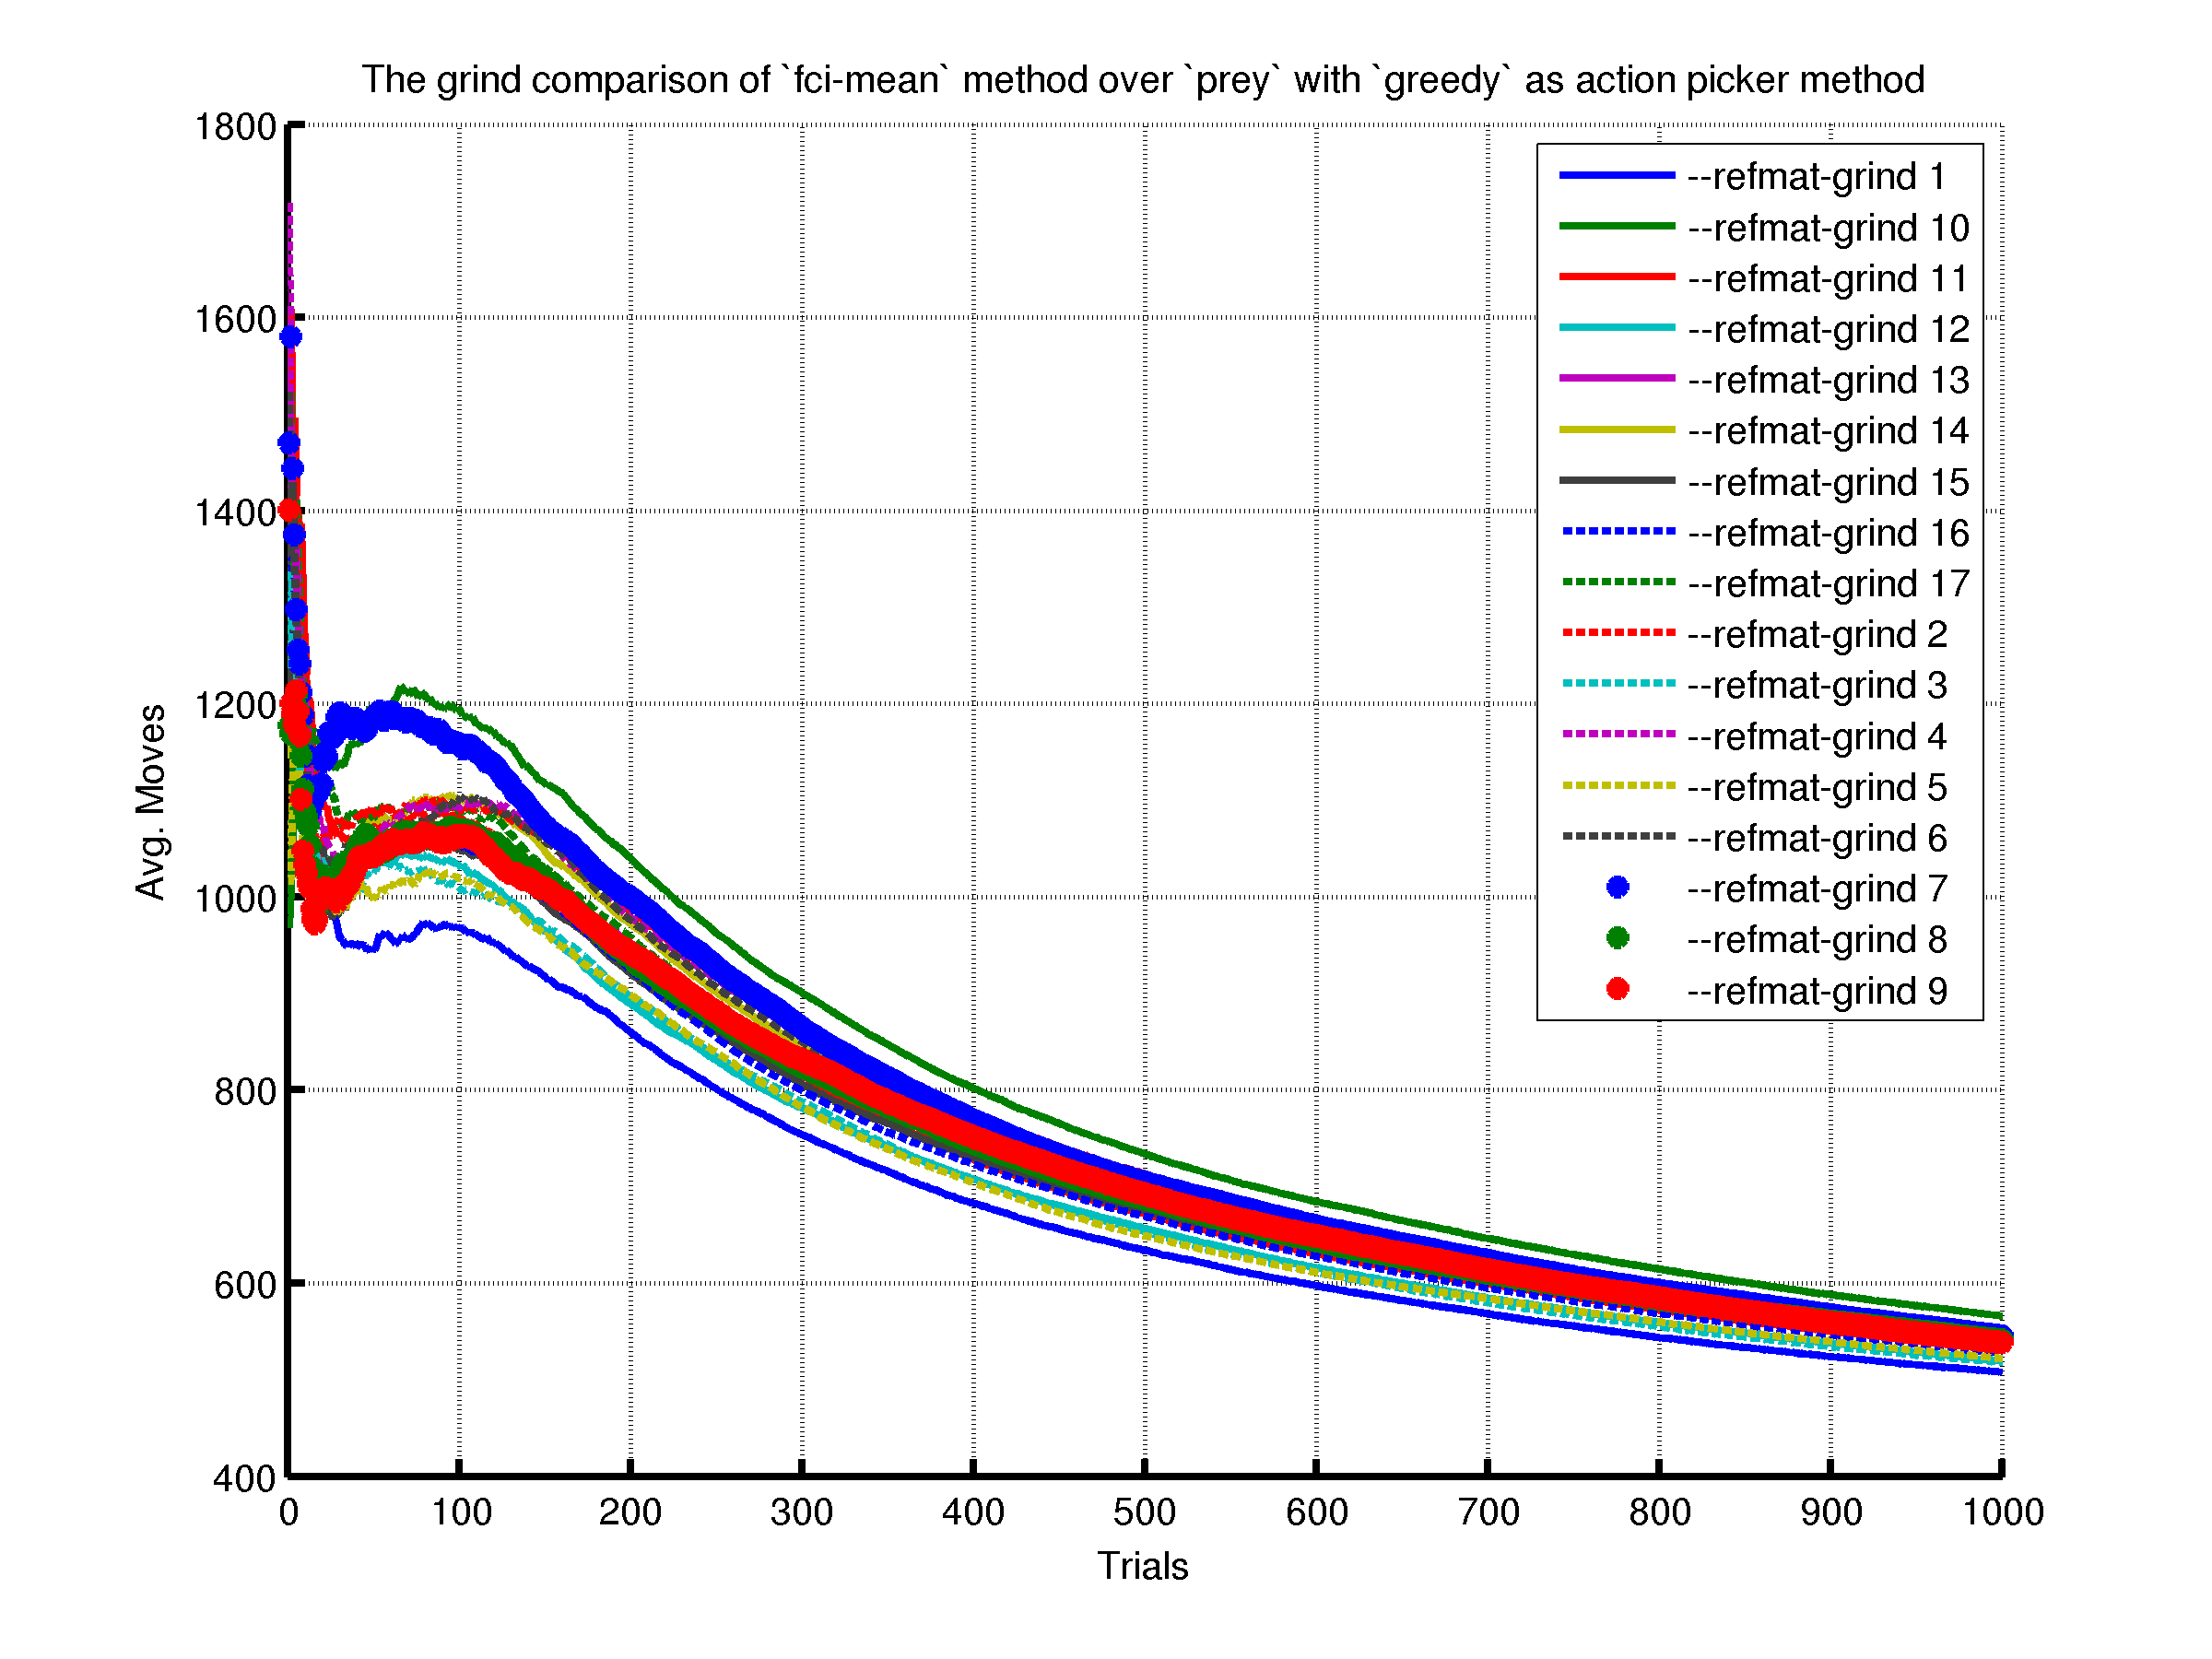
\includegraphics[width=.47\textwidth]{boltzmann/pref/refmat/env/prey/fci-mean/prey-fci-mean-grind-compare.png}}
     {\lr{Mean($\cdot$)}}
\\
\subf{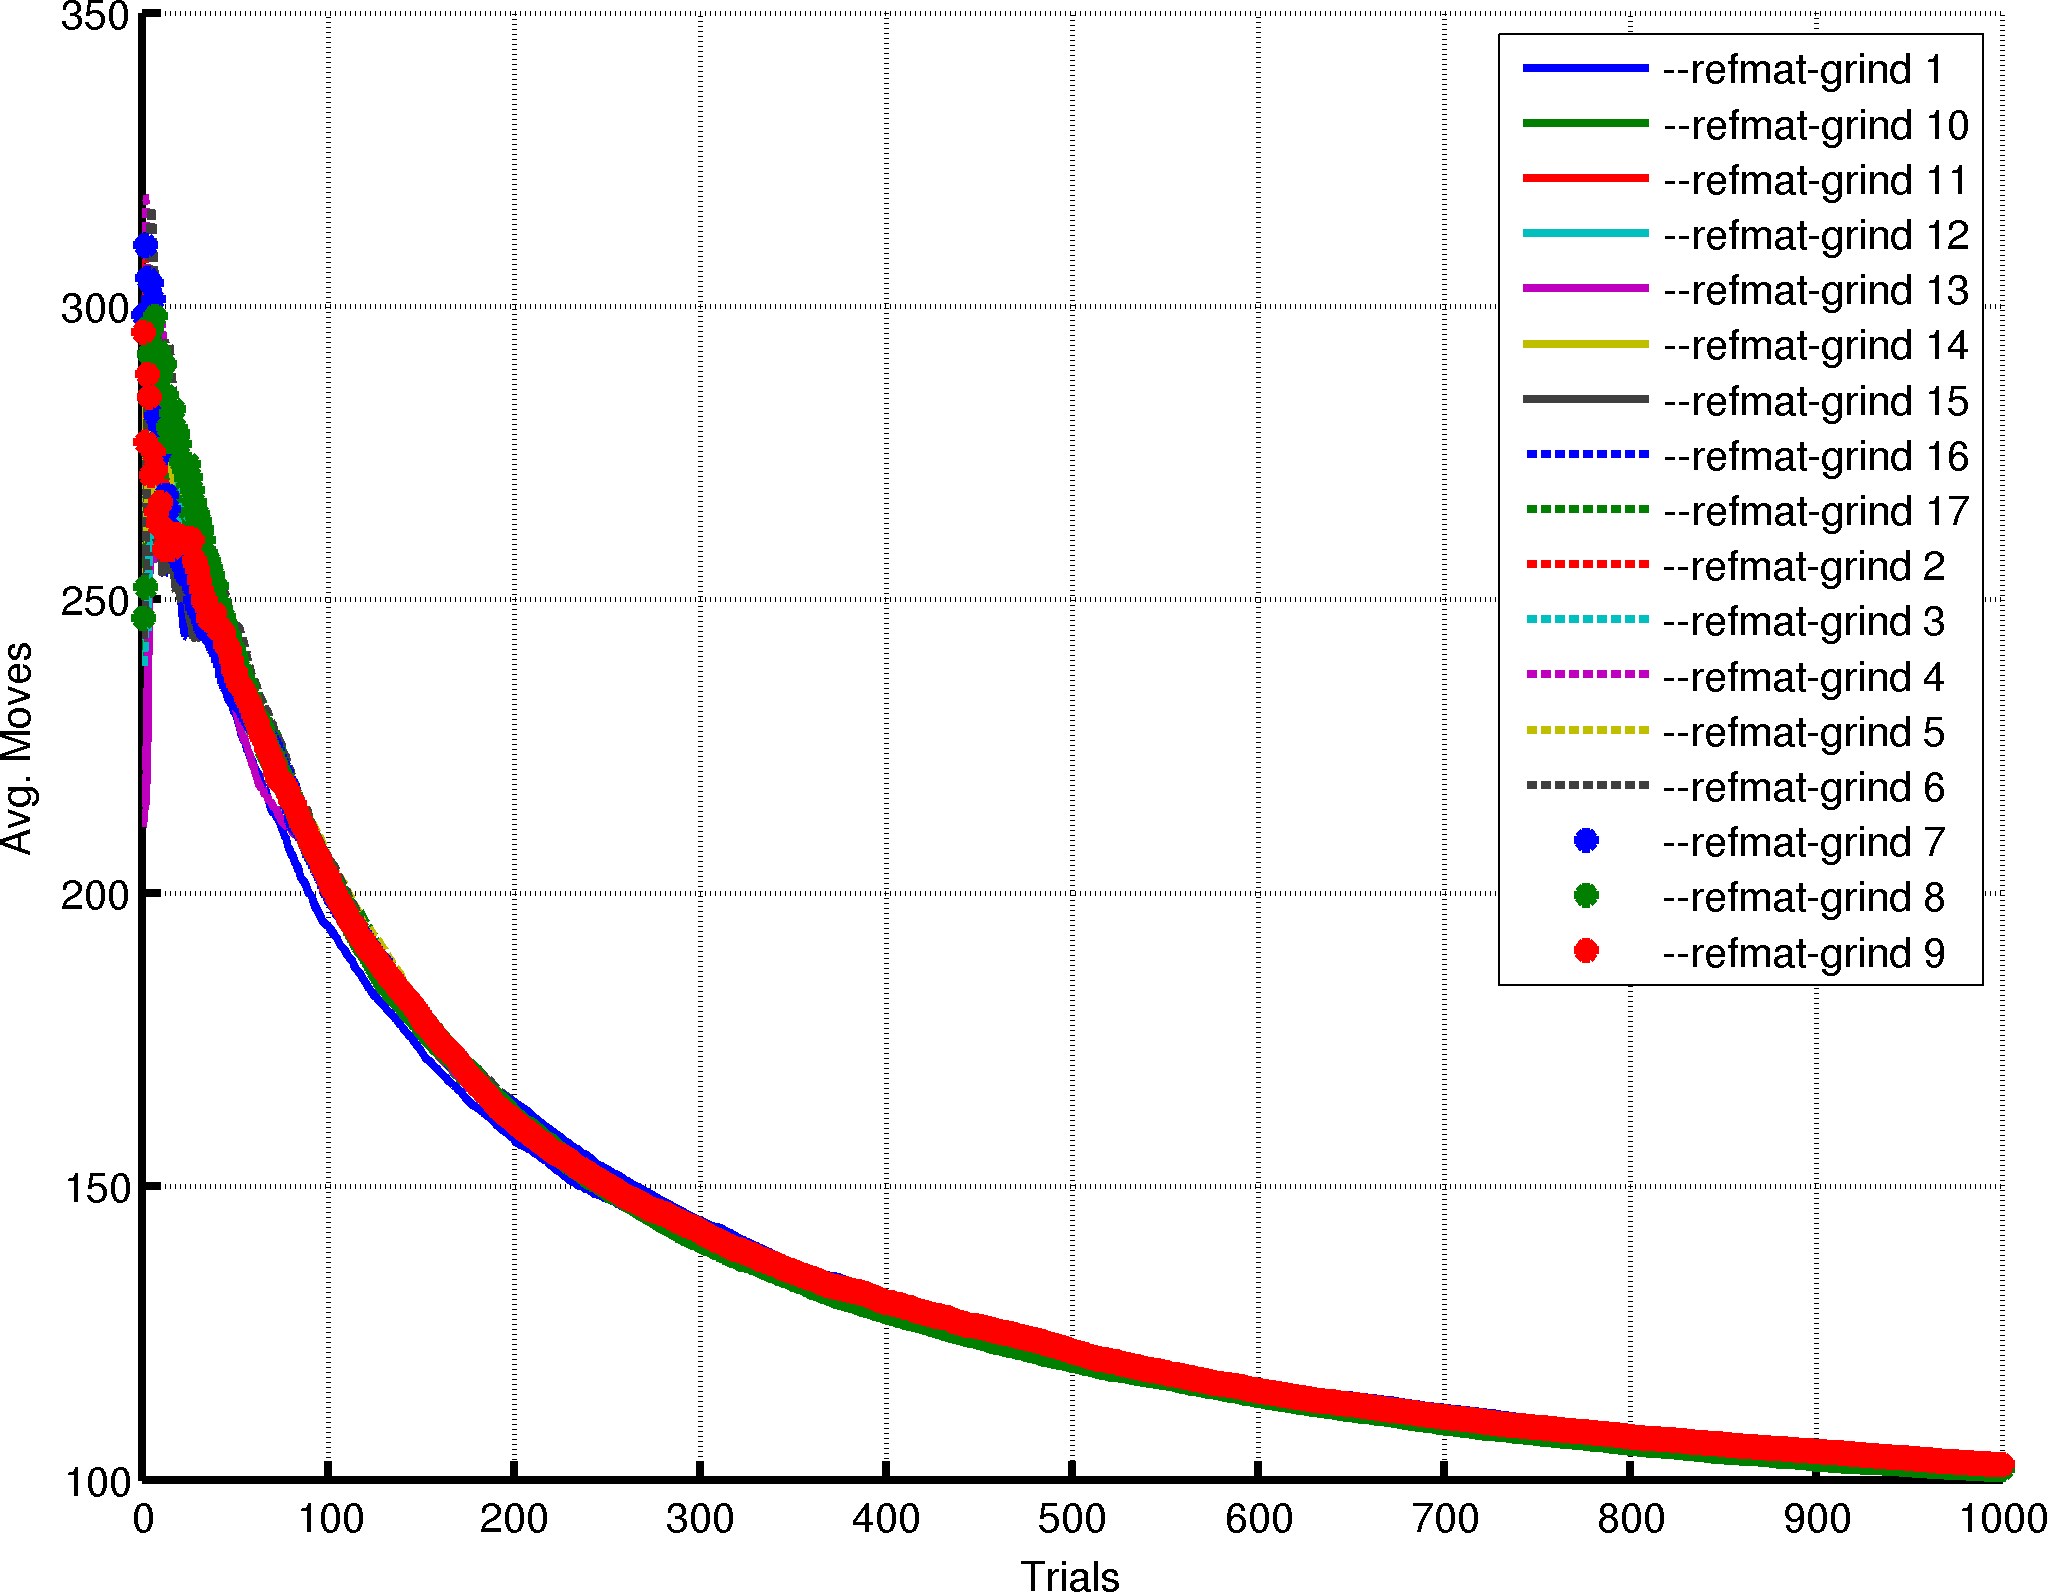
\includegraphics[width=.47\textwidth]{boltzmann/pref/refmat/env/prey/fci-k-mean/prey-fci-k-mean-grind-compare.png}}
     {\lr{K-Mean($\cdot$)}}
&
\subf{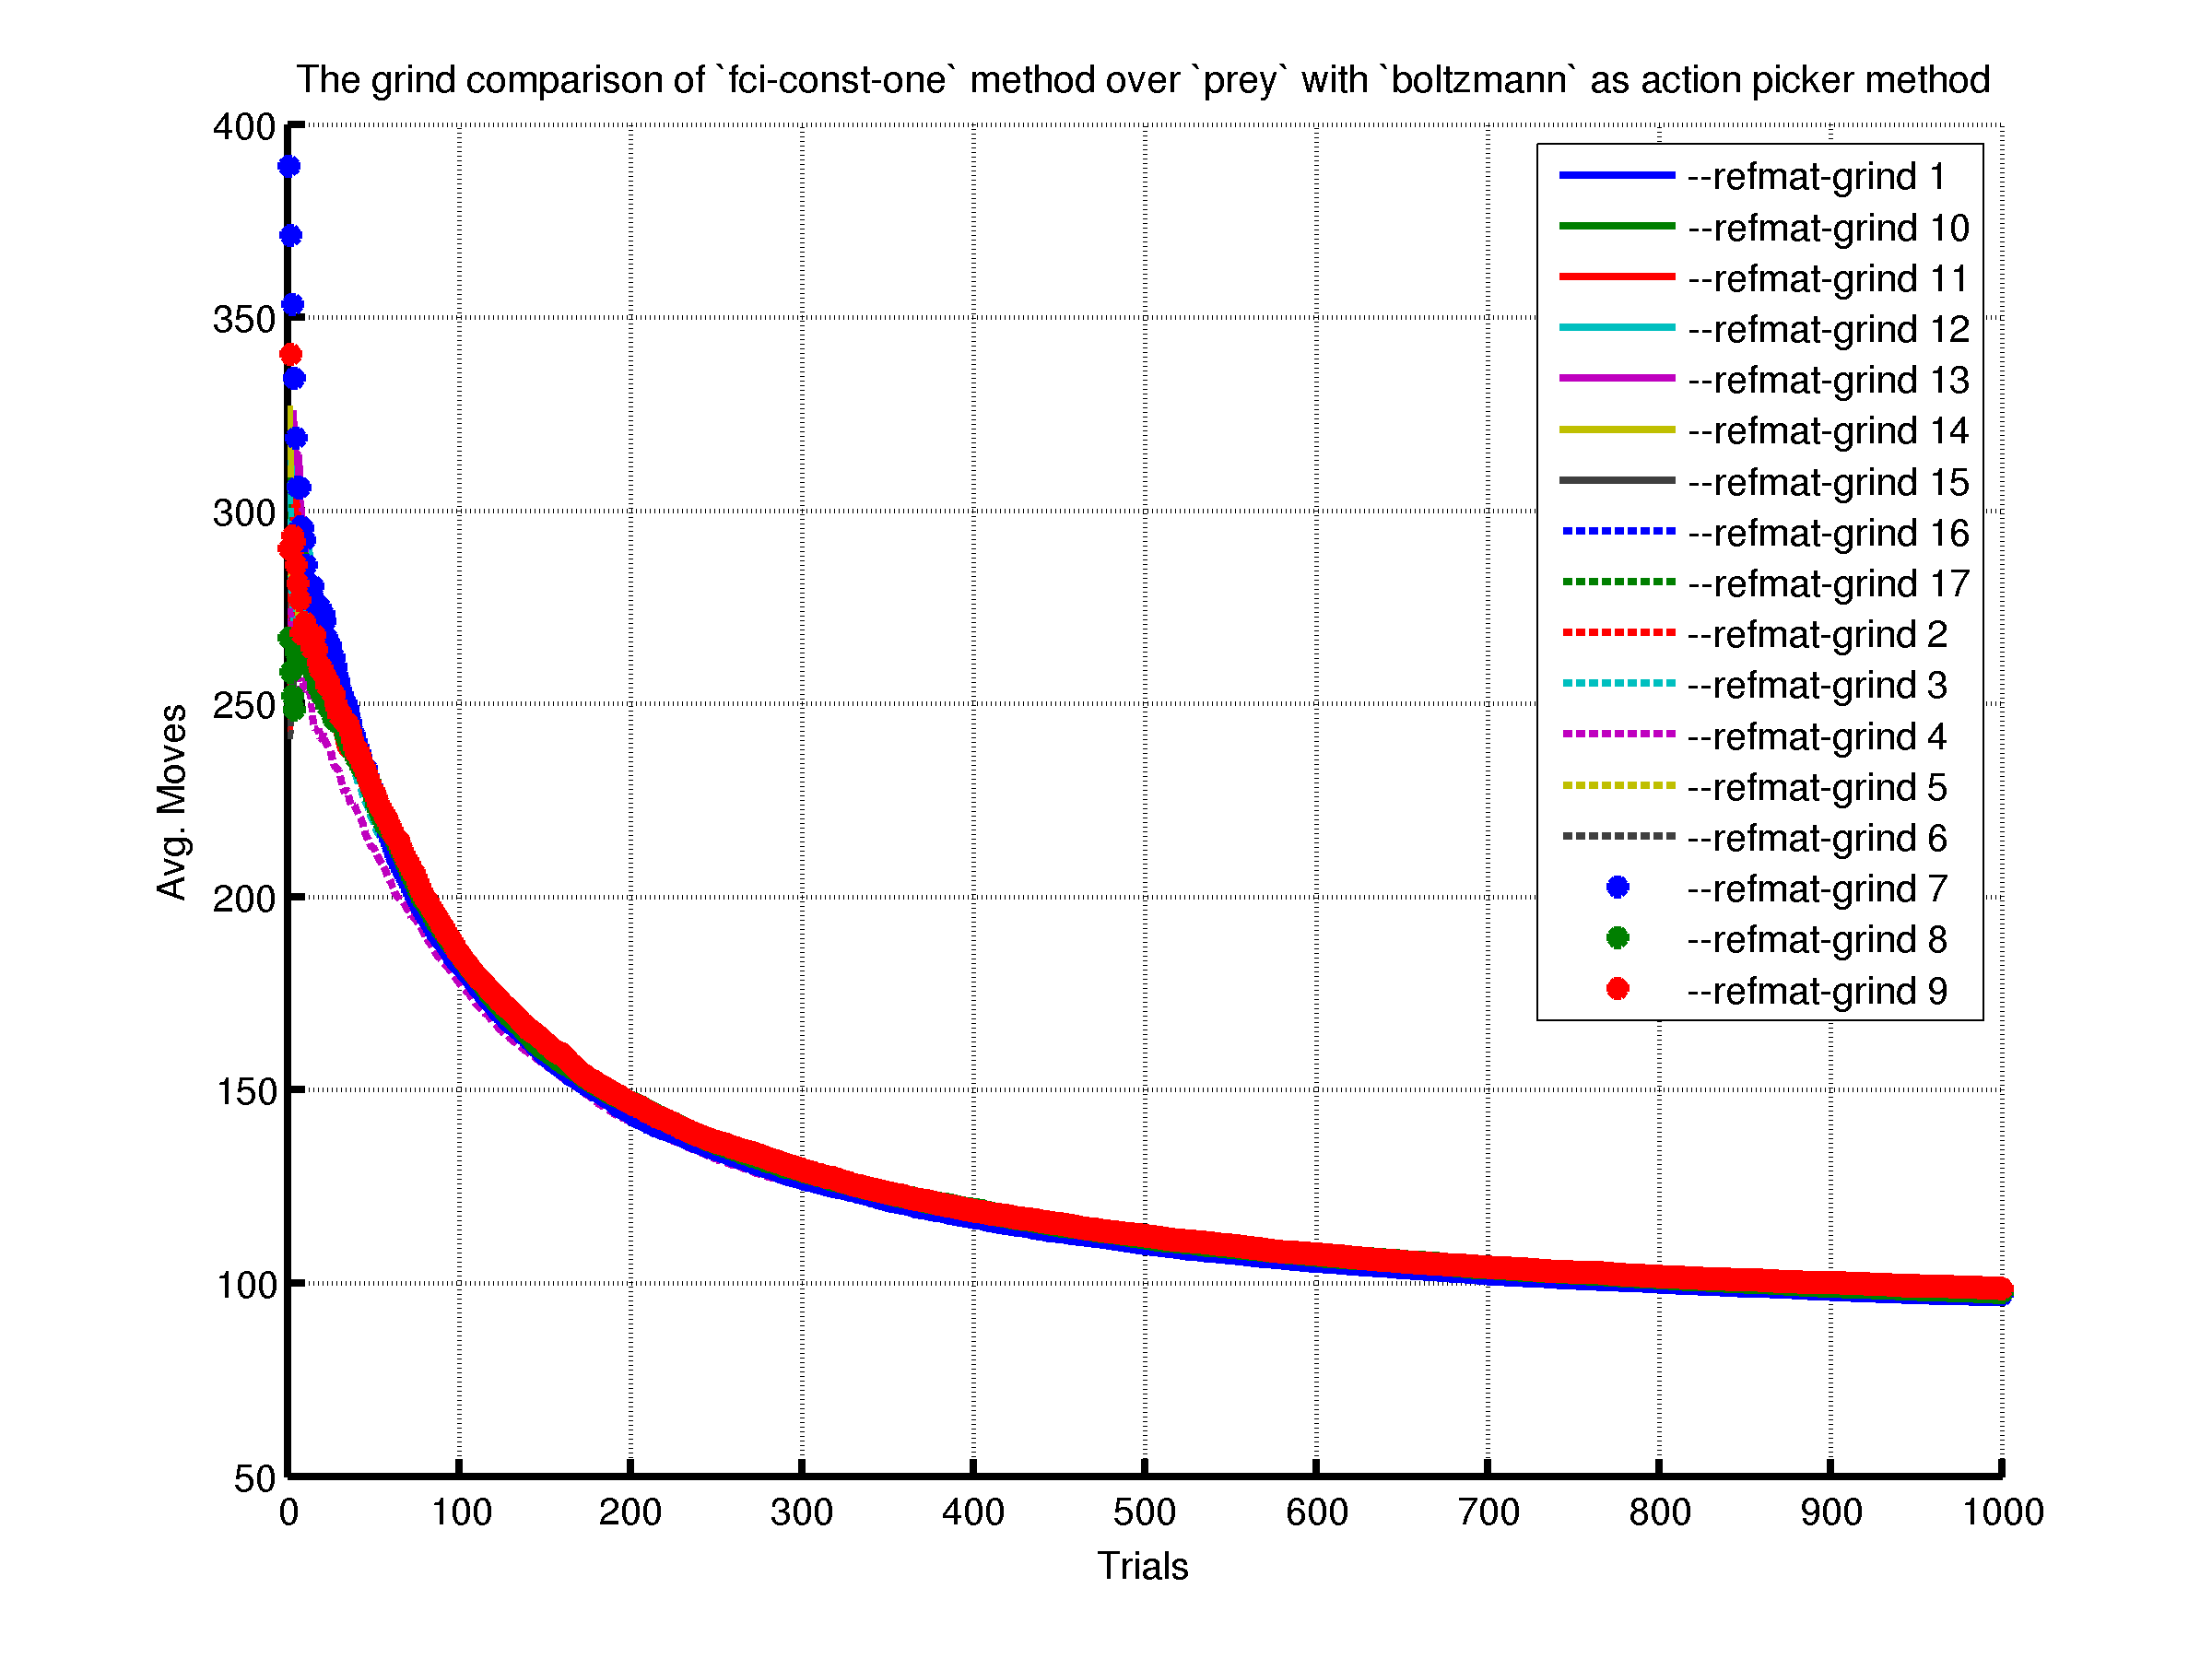
\includegraphics[width=.47\textwidth]{boltzmann/pref/refmat/env/prey/fci-const-one/prey-fci-const-one-grind-compare.png}}
     {\lr{Const-One($\cdot$)}}
\\
\end{tabular}
\end{figure}